% Created 2020-05-25 Mon 17:02
% Intended LaTeX compiler: pdflatex
\documentclass[11pt]{article}
\usepackage[utf8]{inputenc}
\usepackage[T1]{fontenc}
\usepackage{graphicx}
\usepackage{grffile}
\usepackage{longtable}
\usepackage{wrapfig}
\usepackage{rotating}
\usepackage[normalem]{ulem}
\usepackage{amsmath}
\usepackage{textcomp}
\usepackage{amssymb}
\usepackage{capt-of}
\usepackage{hyperref}
\usepackage{minted}
\usepackage{/home/ryan/Dropbox/profiles/Templates/LaTeX/ScreenStyleDV}
\author{Ryan Greenup}
\date{\today}
\title{Analysis of COVID Data}
\hypersetup{
 pdfauthor={Ryan Greenup},
 pdftitle={Analysis of COVID Data},
 pdfkeywords={},
 pdfsubject={},
 pdfcreator={Emacs 27.0.91 (Org mode 9.4)}, 
 pdflang={English}}
\begin{document}

\maketitle
\tableofcontents


\section{Introduction}
\label{sec:org956f2bb}
On December 31st 2019 a report regarding a case of a noteworthy viral pneumonia
was reported in Wuhan, China, this was later found to be a result of a new
strain of virus named \emph{Sars-CoV2}, the disease caused by such an infection,
usually resulting in viral pneumonia, is known as \emph{Corona Virus Disease 2019}
(\emph{COVID-19}). The outbreak of this disease was declared a Public Health
Emergency of International Concern on the 30th January 2020.
\cite{worldhealthorganization2020}

A data set detailing the location, deaths, tests and cases related to the
\emph{COVID-19} pandemic has been made available through the website \emph{Our World in
Data} \cite{ritchie2020}, documented in this report is a visual analyis
performed entirely using the \emph{Free Software} \footnote{Free as in speech and beer} \textbf{\emph{R}} \cite{rcoreteam2020}
primarily with the \texttt{ggplot2} package \cite{wickham2016} (see listing \ref{orgc761d89} in the
appendix).

\section{Chloropleth Map}
\label{sec:org335e89d}
A Chloropleth map of the number of deaths can offer an insight into the impact
that the disease has had with respect to individual countries.

The Total deaths should be scaled relative to the population of the country,
that way countries with a smaller and sparser population will still be
represented by the visualisation (this is quite important given that many
countries such as Italy have a small population compared to the US and much of
Asia \cite{2020n}).

A worldwide Chloropleth map visualising the total number of deaths attributed to
\emph{COVID-19} is shown in figure \ref{fig:orgbde4873} and a Europe-centric visualisation is shown
in figure \ref{fig:org8276add}.

\subsection{Technical Details}
\label{sec:orgb8553bf}
\subsubsection{Preliminary}
\label{sec:org87a2ce8}
\begin{enumerate}
\item Load Packages and Data
\label{sec:org39241de}

Before any analysis can be undertaken it is necessary to load the necessary libraries within \textbf{\emph{R}}, this can be simplified by using a package manager as shown in listing \ref{org8d57e1b}.

\begin{listing}[htbp]
\begin{minted}[]{r}
 if (require("pacman")) {
    library(pacman)
  }else{
    install.packages("pacman")
    library(pacman)
  }
  pacman::p_load(xts, sp, gstat, ggplot2, rmarkdown, reshape2, ggmap,
                 parallel, dplyr, plotly, tidyverse, reticulate, UsingR, Rmpfr,
                 swirl, corrplot, gridExtra, mise, latex2exp, tidyverse, xts, maptools, plyr, ggplot2, maps, viridis)

mise()

\end{minted}
\caption{\label{org8d57e1b}Load the necessary libraries for analysis.}
\end{listing}

\item Load the Data
\label{sec:orgba27346}

Next the data set must be loaded into \textbf{\emph{R}}, this is shown in listing \ref{org5b07650}.

\begin{listing}[htbp]
\begin{minted}[]{r}
covid <- read.csv("/home/ryan/Notes/DataSci/Visual_Analytics/Assessment2/owid-covid-data.csv")

\end{minted}
\caption{\label{org5b07650}Load the data into R}
\end{listing}
\end{enumerate}

\subsubsection{Woldwide Map}
\label{sec:org3a2b75d}
In order to produce a chloropleth map the data must be aggregated in order to retrieve the total number of
deaths, this can be acheived by taking the maximum of the total deaths across
countries (the total number of death rates will be a strictly positive and
monotone trend, otherwise the outbreak would be an entirely different type of
pandemic!), this can be performed by using the \texttt{aggregate} function as
demonstrated in listing \ref{org420cba7}.

\begin{listing}[htbp]
\begin{minted}[]{r}
fatalprop <- aggregate(total_deaths_per_million ~ location, covid, max)
## Order the Values in Descending Order
fatalprop <- fatalprop[order(-fatalprop$total_deaths_per_million),]
## Rename USA
covid$location[covid$location=="United States"] <- "USA"
\end{minted}
\caption{\label{org420cba7}Use Aggregate to aggregate total number of deaths}
\end{listing}


It is next necessary to rename \texttt{location} to \texttt{region} so map data will be
consistent with the provided data set, this is shown in listing \ref{org44f7f71}.

\begin{listing}[htbp]
\begin{minted}[]{r}
## Rename to facilitate joining with map
names(fatalprop) <- c("region", "total_deaths_per_million")
\end{minted}
\caption{\label{org44f7f71}Rename Features for consistency}
\end{listing}

For a broad overview of the data, small regions such as San Marino and Belgium
will not be visible and will skew the colour pallete, so instead they should be removed
and instead a seperate plot of Europe will be created as shown in figure \ref{fig:org8276add}, this removal is performed in
listing \ref{orgef197ce}.

\begin{listing}[htbp]
\begin{minted}[]{r}
## San Marino will be shown by italy and this skews the results
## Belgium and San Marino are very hard to visualise from above
## They skew the rsults and so will be removed.
fatalprops <- fatalprop %>% filter(region!="San Marino")
fatalprops <- fatalprop %>% filter(region!="Belgium")
\end{minted}
\caption{\label{orgef197ce}Filter out small dense regions to prevent scale issues}
\end{listing}


Next it is necessary to retrieve map data, this can be done using the \texttt{map\_data}
function, this data may then be combined by region with the provided data set
using the \texttt{left\_join} function, this is shown in listing \ref{org4e31ba3}.

\begin{listing}[htbp]
\begin{minted}[]{r}
## Retrieve the map data
some_maps <- map_data("world", region = fatalprops$location)

## Join the Data Frames Together
fatalmap <- left_join(fatalprops, some_maps, by = "region")
\end{minted}
\caption{\label{org4e31ba3}Combine Map Data with Provided Data}
\end{listing}

Finally this data frame can be plotted by using \texttt{ggplot2} and the \texttt{geom\_map}
layer, modifying the \texttt{theme} layer will allow for a natural background to be implemented,
this is demonstrated in listing \ref{orgea1e218} and the output is provided in figure \ref{fig:orgbde4873}.

\begin{listing}[htbp]
\begin{minted}[]{r}
wmp <- ggplot(fatalmap, aes(map_id = region)) +
  geom_map(map = fatalmap,  color = "grey", aes(fill = total_deaths_per_million), lwd = 0.1, alpha = 0.6)+
  expand_limits(x = fatalmap$long, y = fatalmap$lat)+
  scale_fill_gradient(high = "darkred", low = "white") +
  guides(fill = guide_legend("Total Deaths \n per Million")) +
   # Change the colors of background
   # and the color of grid lines to white
   theme(
     panel.background = element_rect(fill = "lightblue",
                                     colour = "lightblue",
                                     size = 0.5, linetype = "solid"),
     legend.position = c(0.6, 0.1),
     legend.direction = "horizontal",
     legend.background = element_rect(fill = "white", size = 0.1, colour = "darkblue", linetype = "solid")) +
   labs(x = "Longitude", y = "Latitude", title = TeX("Total Deaths Attributed to \\textit{COVID-19}"))
#   geom_text(data = region_lab_df, aes(y = lat, x = long, label = region), size = 1)
wmp

\end{minted}
\caption{\label{orgea1e218}use \texttt{ggplot2} to create a chloropleth map from data, output in figure \ref{fig:orgbde4873}}
\end{listing}


\begin{figure}[htbp]
\centering
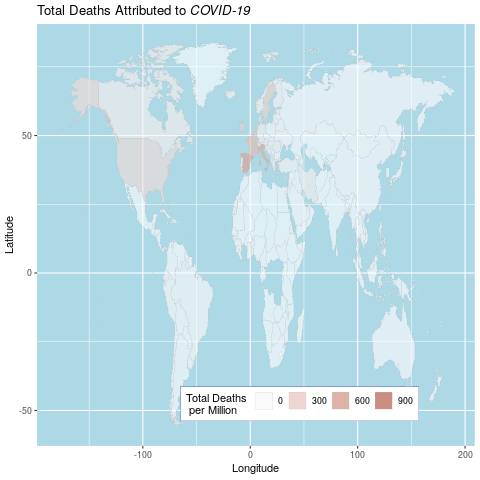
\includegraphics[width=16cm]{FirstChALL.png}
\caption{\label{fig:orgbde4873}Chloropleth map of total deaths attributed to \emph{COVID-19} (per Million people)}
\end{figure}

A bubble overlay may also be implemented in order make clearer the spread of cases (see section \ref{org8f1cfd9} for a brief literature review), it is necessary however to adjust the \emph{USA} location to represent the mainland population centre in order make the visualisation more effective. This is demonstrated in listing \ref{orgdf4f16f} and shown in figure \ref{fig:orga1d9f48}

\begin{listing}[htbp]
\begin{minted}[]{r}

# Compute the centroid as the mean longitude and lattitude
# Used as label coordinate for country's names
region_lab_df <- some.eu.maps %>%
  group_by(region) %>%
  summarise(long = mean(long), lat = mean(lat)) %>%
    full_join(aggregate(total_deaths_per_million ~ region, fatalmap, mean))
# Manually Adjust US to be population Centre
region_lab_df[region_lab_df$region == "USA",]$long <- -92.47
region_lab_df[region_lab_df$region == "USA",]$lat <- 37.37


wmp +
  scale_size_continuous(range = c(1, 9), name = "Total Number \n of Deaths") +
   guides(size = FALSE) +
   geom_point(data = region_lab_df, aes(y = lat, x = long, size = total_deaths_per_million), alpha = 0.5, col = "purple")
\end{minted}
\caption{\label{orgdf4f16f}use \texttt{ggplot2} to create a chloropleth map from data, output in figure \ref{fig:orgbde4873}}
\end{listing}

\begin{figure}[htbp]
\centering
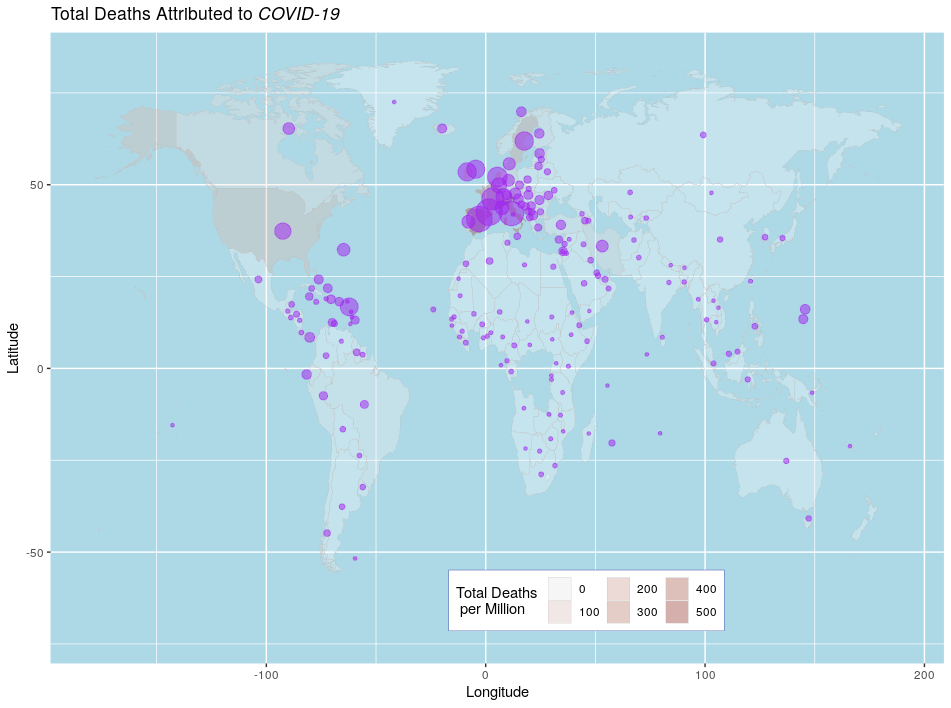
\includegraphics[width=16cm]{FirstChAllbub.png}
\caption{\label{fig:orga1d9f48}Chloropleth map with bubble overlay to aid in case visualisation}
\end{figure}

\subsubsection{Europe Centric}
\label{sec:orgfbfc7a1}
The chloropleth map clearly shows that the disease has caused significiantly more fatalities
per capita in Europe and so the plot will be adjusted central to Europe.

As before it is necessary to rename the features of the dataset, however in this
instance small European countries such as Belgium should be retained (San marino
is a very small italian provice that isn't detectable in the visualisation and
skews the pallete, for this reason it will be removed), this is demonstrated in
listing \ref{orga17bfdd}.

\begin{listing}[htbp]
\begin{minted}[]{r}
## Rename to facilitate joining with map
names(fatalprop) <- c("region", "total_deaths_per_million")

## San Marino will be shown by italy
 fatalprop <- fatalprop %>% filter(region!="San Marino")
\end{minted}
\caption{\label{orga17bfdd}Rename the features of the data and remove San Marino}
\end{listing}

In this map it will be desirable to have labels for the European countries
(whereas this would have made the worldwide map too busy), so this will be
implemented by using \texttt{dyplyr} to generate a second data set as shown in listing
\ref{orgc0543c1} which can then be used to generate a plot with the \texttt{ggrepel} add on as shown in listing \ref{orgf7a336d}, this
produces the output shown in figure \ref{fig:org8276add}, bubbles were also implemented in order to help visualise the number of relative cases.

\begin{listing}[htbp]
\begin{minted}[]{r}
fatalmap <- left_join(fatalprop, some.eu.maps, by = "region")

## Filter out only Europe
fatalmap <-  fatalmap %>%
  filter(30 <  lat & lat < 65) %>%
  filter(-30 <  long & long < 35)

## Create Label Data Frame
region_lab_df <- fatalmap %>%
  dplyr::group_by(region) %>%
  dplyr::summarise(long = mean(long), lat = mean(lat)) %>%
   full_join(aggregate(total_deaths_per_million ~ region, fatalmap, mean))
\end{minted}
\caption{\label{orgc0543c1}use \texttt{dplyr} to reduce the plot size and create a data frame of country labels}
\end{listing}


\begin{listing}[htbp]
\begin{minted}[]{r}
library(ggrepel)
ggplot(fatalmap, aes(map_id = region, label = region)) +
  geom_map(map = fatalmap,
           aes(fill = total_deaths_per_million),
           color = "white") +
  geom_point(data = region_lab_df, aes(y = lat, x = long, size = total_deaths_per_million), alpha = 0.45, colour = "blue", stroke = 1, fill = "white", shape = 21) +  scale_size_continuous(range = c(1, 25), name = "Total Number \n of Deaths") +
  guides(size = FALSE) +
  expand_limits(x = fatalmap$long, y = fatalmap$lat) +
  scale_fill_viridis_c(option = "C") +
  scale_fill_gradient(high = "darkred", low = "white") +
  guides(fill = guide_legend("Total Deaths \n per Million")) +
  # Change the colors of plot panel background to lightblue
  # and the color of grid lines to white
  theme(
    panel.background = element_rect(
      fill = "lightblue",
      colour = "lightblue",
      size = 0.5,
      linetype = "solid"
    ),
    legend.position = c(0.1, 0.6),
    legend.direction = "vertical",
    legend.background = element_rect(
      fill = "white",
      size =
        1.1,
      colour = "darkblue",
      linetype = "solid"
    )
  ) +
  labs(
    x = "Longitude",
    y = "Latitude",
    title = TeX("Total Deaths Attributed to \\textit{COVID-19}")
  ) +
  geom_text_repel(
    data = region_lab_df,
    aes(y = lat, x = long, label = region),
    size = 2,
    col = "black",
    nudge_y = 0.7,
    nudge_x = -0.5,
    min.segment.length = 0.6,
    force = 2
  )
\end{minted}
\caption{\label{orgf7a336d}Generate a Chloropleth map centred on Europe using \texttt{ggplot2}}
\end{listing}


\begin{figure}[htbp]
\centering
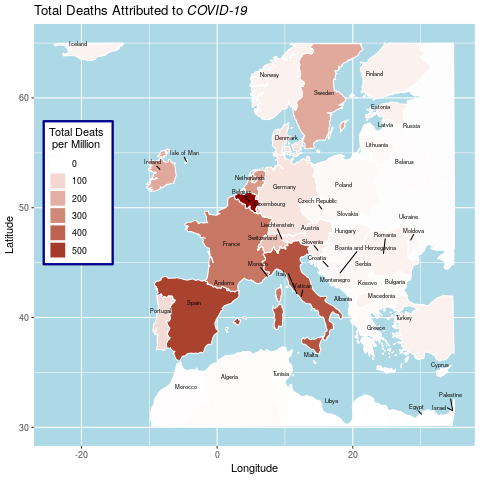
\includegraphics[width=16cm]{SecChEur.png}
\caption{\label{fig:org8276add}Europe Centred Chloropleth of Deaths Attributed to \emph{COVID-19}}
\end{figure}

\subsection{Discussion}
\label{sec:org75a6c83}
\subsubsection{Worldwide}
\label{sec:org13220d1}
The first plot appears to show a very limited amount of difference in deaths
attributable to \emph{COVID-19} across regions other than North America and
Europe.

While first-world countries such as New Zealand and Australia are
somewhat insulated from the disease by virtue of geography and population
density, it's striking that much of Asia and Russia have such low levels of
disease incidence.

This could be attributed to the fact that a more power-centric regime such as in
China, Russia, North Korea, etc. may have more capacity to:

\begin{enumerate}
\item Diminish the spread of the disease by implementing
policy decisions,
\begin{enumerate}
\item whereas countries such as the US and Europe have a much higher expectation
of civil liberties and hence much lower tolerance for government intervention.
\end{enumerate}
\item Control the spread of information for want of international reputation.
\begin{enumerate}
\item In saying that though research suggests that under-reporting has even
occured in countries such as the US \cite{sood2020} so such under-reporting
could merely be incidental.
\end{enumerate}
\end{enumerate}

A similar disease, \emph{MERS}, emerged in 2012 in Middle-Eastern Regions
\cite{woodley2020} and a Korean outbreak of the \emph{MERS} disease occured in 2015
\cite{serrano2015}, these outbreaks likely prepared Korea, the Middle East and
other Asian regions for an outbreak which helps explain the dichotomous
nature of the deaths attributable to \emph{COVID-19} for those Countries.

\subsubsection{Europe}
\label{sec:orge45e1ab}
A closer look at Europe shows that Belgium and Italy have been the most affected
by this disease, it isn't very clear why those regions have been impacted so
significantly, particularly considering the comparatively permissive borders
within the \emph{EU}, but this could be indicative of policy decisions and warrants
further research.

\subsection{Advantages compared to other methods}
\label{sec:orgab47f26}
A Chloropleth map provides a very clear way to visualise the occurence of
disease in a geographical sense, in contrast to other methods such as scatter
plots, heatmaps and bar charts, the chloropleth map provides a clear way to
distinguish the impact of the disease on individual countries.

Chloropleth maps also allow trends across regions to be easily identified, e.g.
figure \ref{fig:org8276add} shows how severe the outbreak is in \emph{Europe} relative to other
regions, this might be lost in abstraction when using other visualization methods.

The discrete distinction between countries, a fundamental component of a
chloropleth map, is desirable because it is consistent with the independent
legislatures accross countries, this allows for a comparison of the impact
that policy decisions may or may not have on a region.

\subsection{Disasadvantages}
\label{sec:org659d7a5}
When maps are projected into a 2D plane they are necessarily distorted, this
distortion can impact how spread the data appears to be.

A chloropleth map can make it hard to compare metrics between to regions in any
specific sense, for this a more appropriate visualization could be for instance a bar chart.
\subsection{Literature review of related work}
\label{sec:org4a86e6b}
The \emph{John Hopkins Coronavirus Dashboard}  \cite{2020o} implemented bubbles to
visualise the number of cases, a screenshot of this is provided in the appendix
at figure \ref{fig:org2e5afd2}, this was a part of the motivation for implementing bubbles in
the chloropleth map because the visualization was so much more \emph{striking} and
promoted pre-attentive processing of the information.

\label{org8f1cfd9} In his blog, Kenneth Field produced chloropleth and bubble-map charts
detailing the spread of \emph{COVID-19}, with however, a focuse on China, \cite{field2020} these
plots were very similar to those produced in this report, however the legend for
the bubble plot was very nicely implemented and can be seen in figure \ref{fig:orge888b39} of
the appendix. He also produced an example illustrating why the use of a heatmap
or contour map can make for a poor visualisation of cases due to the difficulty
in interpreting the visualization compared to a bubble chart, for this reason a
bubble chart was used in this report and a heatmap was not implemented.

A paper in the publication \emph{Environment \& Planning A} suggested using a
cartogram to visualise the spread of disease, there example is provided in
figure \ref{fig:orgb7dd52e} of the appendix. \cite{gao2020} Although the cartogram is visually
quite appealing and easy to read, it is difficult to interpret quickly, the
visualisation does not promote pre-attentive processing, for this reason the
visualisation strategy was not implemented.

\section{Time Series}
\label{sec:org4957c46}
\subsection{Implementation}
\label{sec:org7595a19}
Time series charts can be an effective way to visualise the behaviour of a value
over time, for this dataset however, two modifications will be implemented in
order to make the trends more distinct.

\subsubsection{Log Scale}
\label{sec:orge5a6140}
The spread of disease over time can often be described by an exponential model as
demonstrated in equations \eqref{exp1} and \eqref{exp2}, for this reason the use of
a \(\log\) -scale will linearise trends and so the use of a \(\log\) -scale will make
it easier to compare the rates of population change between different countries.



\begin{align}
  \frac{\mathrm{d} p}{\mathrm{d} t} \propto p &\implies p = Ce^{kt} \quad \exists k,c \in \mathbb{R} \label{exp1} \\
  \frac{\mathrm{d} p}{\mathrm{d} t} \propto p \wedge    \frac{\mathrm{d} p}{\mathrm{d} t} \propto (N-p) &\implies p = \frac{ke^{Nt}}{1-ke^{Nt}} \quad \exists k \in \mathbb{R}, N \in \mathbb{R^+} \label{exp2}
\end{align}

\subsubsection{Adjust Zero}
\label{sec:orgfa6e39c}
In addition to a \(\log-\) scale, \emph{sliding} the data to be relative to the number
of days since the first case can allow the trends of the data to be compared, A
similar technique was implemented by \emph{John Hopkins University} in a
visualisation published in \emph{The Guardian} \cite{gutierrez2020}. \label{orgb846a90} Here the
number of cases has been considered from the date of the first case, however,
figure \ref{fig:org4bbeb34} shows the trend from the date of the 100th case, while it appears to
line the countries up better the loss of information was undesirable.
\subsection{Technical Details}
\label{sec:org422c64f}
\subsubsection{Preliminary}
\label{sec:org7ab654c}
In order to log scale the data the \texttt{mutate} function from the \texttt{dplyr} package
was used on data transformed into \emph{wide} format by using the \texttt{pivot\_wider}
function, this is shown in listing \ref{org4691f98}.

Sliding the date back to the number of cases however was a little more difficult
and required the use of a \texttt{for} loop to iterate the \texttt{lead} function over each
column (where each column, after transformation with \texttt{dplyr}, represented the
value for a country), this is demonstrated in listing \ref{org4691f98} with an example of the
produced \emph{tidy} data provided in table \ref{tab:orge7eb163}; the code to produce the plot is
demonstrated in listing \ref{org5bb4fe3}, the output of which is provided in figure \ref{fig:org4bbeb34}.

Rather than using a line plot or a scatter plot, a \texttt{loess} model was placed ontop of semi-opaque points, this is to enhance the continuity of the visualisation. The \emph{Gestalt Laws} provide that continuous shapes are easier for readers to interpret \cite{staudinger2011} and for this reason the the overlay was implemented, to aid the reader in delineating between the different countries in a plot.

Plots with many colours mapped to categorical variables can be difficult to interpret \cite{wilson2017,rost2018}, for this reason less than 10 countries were compared on the same plot.

\begin{listing}[htbp]
\begin{minted}[]{r}
cv <- as_tibble(covid)
cv <- cv %>%
  mutate(date = as.Date(date))
cv <- cv[order(cv$date),]

# interested_locations <- c("Australia", "USA", "Italy", "Germany", "Belgium", "United Kingdom", "New Zealand", "Japan", "China")
interested_locations <- c("Australia", "USA", "Italy", "Germany", "Russia", "South Korea", "United Kingdom")

cv <- cv %>%
  filter(location %in% interested_locations) %>%
  filter(total_cases_per_million > 1) %>%
  mutate(total_cases_per_million = log10(total_cases_per_million)) %>%
  dplyr::select(date, total_cases_per_million, location) %>%
  pivot_wider(names_from = location, values_from = total_cases_per_million)


for (i in 2:ncol(cv)) {
  ## Slide the Columns up and put the NA at the end
cv[,i] <-   pull(cv, i) %>%
  lead(cv[,i] %>%
         is.na() %>%
         sum())
 ## Replace the date with the number of days
cv$date <- seq_len(nrow(cv))
}

cv <- cv %>%
 pivot_longer(names(cv)[-1], names_to = "location", values_to = "total_cases_per_million")
\end{minted}
\caption{\label{org4691f98}Use \texttt{dplyr} to transform the data as shown in table \ref{tab:orge7eb163}, this can then be passed to ggplot as shown in listing \ref{org5bb4fe3}}
\end{listing}

\begin{table}[htbp]
\caption{\label{tab:orge7eb163}Top few rows of the \emph{tidy} data set created from listing \ref{org4691f98}.}
\centering
\begin{tabular}{rlr}
\emph{\textbf{Date}} & \emph{\textbf{Location}} & \emph{\textbf{Total Cases Per Million}}\\
1 & South Korea & 0.193\\
1 & Italy & 0.116\\
1 & Australia & 0.00860\\
1 & Germany & 0.122\\
1 & United Kingdom & 0.0976\\
1 & USA & 0.00903\\
1 & Russia & 0.00303\\
2 & South Korea & 0.480\\
2 & Italy & 0.339\\
2 & Australia & 0.0558\\
\end{tabular}
\end{table}

\begin{listing}[htbp]
\begin{minted}[]{r}
ggplot(cv , aes(y = total_cases_per_million, x = date, col = location, group = location)) +
  geom_point(alpha = 0.3)  +
  geom_smooth() +
  theme_bw() +
  labs(y = "Total Number of Cases (Log-10 Scale)", title = "Log Scaled Total COVID-19 Cases per Million", x = TeX("Days since Case \\textit{#100}")) +
  guides(col = guide_legend("Location"))
#  geom_smooth()
\end{minted}
\caption{\label{org5bb4fe3}Use \texttt{dplyr} to transform the data before plotting with \texttt{ggplot}}
\end{listing}


\begin{figure}[htbp]
\centering
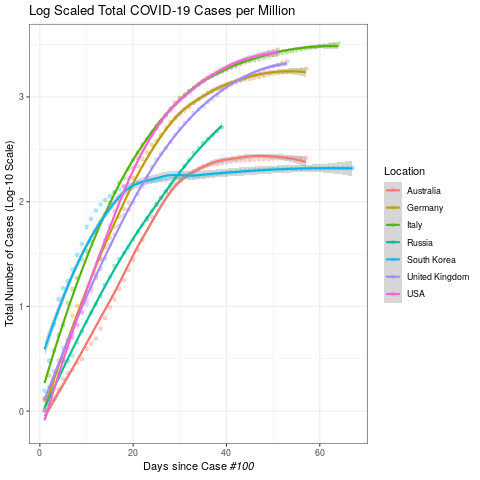
\includegraphics[width=12cm]{FirstTS.png}
\caption{\label{fig:org4bbeb34}Chloropleth map of total deaths attributed to \emph{COVID-19} (per Million people)}
\end{figure}

\subsubsection{Facet Grid}
\label{sec:org747b052}
This plot however does not show all the data made available, the data set also
includes information on the number of tests,cases and deaths resulting from
\emph{COVID-19}, in order to visualise this the \texttt{fact\_grid} layer can be used to
create a multi-scatterplot. first it is necessary to create a data frame, this
can be implemented by repeating the process in listing \ref{org4691f98} for each different
metric but it will also be necessary to add a feature corresponding to that
metric's description, we will also create non-log scaled data as well, this is
demonstrated in listings \ref{org2af87a5} through \ref{org4c22a85}, finally the dataframes are merged
in listing \ref{org58d5812}, the corresponding plot is shown in figure \ref{fig:org542b788}.

\begin{listing}[htbp]
\begin{minted}[]{r}
interested_locations <- c("Australia", "USA", "Italy", "Germany", "Russia", "South Korea", "United Kingdom")

###### Number of Cases
cv <- as_tibble(covid)
cv <- cv %>%
  mutate(date = as.Date(date))
cv <- cv[order(cv$date),]

cv <- cv %>%
  filter(location %in% interested_locations) %>%
  filter(total_cases > 1) %>%
  mutate(total_cases_per_million = log10(total_cases_per_million)) %>%
  dplyr::select(date, total_cases_per_million, location) %>%
  pivot_wider(names_from = location, values_from = total_cases_per_million)

for (i in 2:ncol(cv)) {
  ## Slide the Columns up and put the NA at the end
cv[,i] <-   pull(cv, i) %>%
  lead(cv[,i] %>%
         is.na() %>%
         sum())
 ## Replace the date with the number of days
cv$date <- seq_len(nrow(cv))
}

cv_cases_log <- cv %>%
 pivot_longer(names(cv)[-1], names_to = "location", values_to = "value") %>%
  add_column(subject = "No. of Cases") %>%
  add_column(scale = "Log-10 Scale")

\end{minted}
\caption{\label{org2af87a5}Use \texttt{dplyr} to create a data frame of log scaled cases}
\end{listing}

\begin{listing}[htbp]
\begin{minted}[]{r}

### Number of deaths

cv <- as_tibble(covid)
cv <- cv %>%
  mutate(date = as.Date(date))
cv <- cv[order(cv$date),]

cv <- cv %>%
  filter(location %in% interested_locations) %>%
  filter(total_cases > 1) %>%
   mutate(total_deaths_per_million = log10(total_deaths_per_million)) %>%
  dplyr::select(date, total_deaths_per_million, location) %>%
  pivot_wider(names_from = location, values_from = total_deaths_per_million)

for (i in 2:ncol(cv)) {
  ## Slide the Columns up and put the NA at the end
cv[,i] <-   pull(cv, i) %>%
  lead(cv[,i] %>%
         is.na() %>%
         sum())
 ## Replace the date with the number of days
cv$date <- seq_len(nrow(cv))
}

cv_deaths_log <- cv %>%
 pivot_longer(names(cv)[-1], names_to = "location", values_to = "value") %>%
  add_column(subject = "No. of Deaths") %>%
  add_column(scale = "Log-10 Scale")


\end{minted}
\caption{\label{org51fccd9}Use \texttt{dplyr} to create a data frame of log scaled deaths}
\end{listing}


\begin{listing}[htbp]
\begin{minted}[]{r}
### Number of Tests
cv <- as_tibble(covid)
cv <- cv %>%
  mutate(date = as.Date(date))
cv <- cv[order(cv$date),]
cv <- cv %>%
  filter(location %in% interested_locations) %>%
  filter(total_cases > 1) %>%
  mutate(total_tests_per_thousand = log10(total_tests_per_thousand)-3) %>%
  dplyr::select(date, total_tests_per_thousand, location) %>%
  pivot_wider(names_from = location, values_from = total_tests_per_thousand)

for (i in 2:ncol(cv)) {
  ## Slide the Columns up and put the NA at the end
cv[,i] <-   pull(cv, i) %>%
  lead(cv[,i] %>%
         is.na() %>%
         sum())
 ## Replace the date with the number of days
cv$date <- seq_len(nrow(cv))
}
cv_tests_log <- cv %>%
 pivot_longer(names(cv)[-1], names_to = "location", values_to = "value") %>%
  add_column(subject = "No. of Tests") %>%
  add_column(scale = "Log-10")

cv <- rbind(cv_cases_log, cv_deaths_log, cv_tests_log)
cv %>%
  filter(subject == "deaths")

p_per_cap <- ggplot(cv , aes(y = value, x = date)) +
  geom_point(alpha = 0.3, aes(col = location))  +
   geom_smooth(aes(col = location), size = 0.5) +
  theme_bw() +
  labs(y = TeX("Count (log_{10} Scale)"), title = TeX("log_{10} Scale; Value of \\textit{COVID-19} Statistics over Time"), x = TeX("Days since Case \\textit{#1}"), subtitle = "Counts Per Million of population") +
  guides(col = guide_legend("Location")) +
  facet_grid(rows = vars(subject), scales = "free_y")
p_per_cap
\end{minted}
\caption{\label{orgbed3112}Use \texttt{dplyr} to create a data frame of log scaled deaths, observe thousands is scaled to millions.}
\end{listing}

\begin{listing}[htbp]
\begin{minted}[]{r}
interested_locations <- c("Australia", "USA", "Italy", "Germany", "Russia", "South Korea", "United Kingdom")

###### Number of Cases
cv <- as_tibble(covid)
cv <- cv %>%
  mutate(date = as.Date(date))
cv <- cv[order(cv$date),]

cv <- cv %>%
  filter(location %in% interested_locations) %>%
  filter(total_cases > 1) %>%
# mutate(total_cases = log10(total_cases)) %>%
  dplyr::select(date, total_cases_per_million, location) %>%
  pivot_wider(names_from = location, values_from = total_cases_per_million)

for (i in 2:ncol(cv)) {
  ## Slide the Columns up and put the NA at the end
cv[,i] <-   pull(cv, i) %>%
  lead(cv[,i] %>%
         is.na() %>%
         sum())
 ## Replace the date with the number of days
cv$date <- seq_len(nrow(cv))
}

cv_cases_raw <- cv %>%
 pivot_longer(names(cv)[-1], names_to = "location", values_to = "value") %>%
  add_column(subject = "No. of Cases") %>%
  add_column(scale = "Count")

\end{minted}
\caption{\label{orge5f6201}use \texttt{dplyr} to create a data frame of non-log scaled cases}
\end{listing}

\begin{listing}[htbp]
\begin{minted}[]{r}
### Number of deaths

cv <- as_tibble(covid)
cv <- cv %>%
  mutate(date = as.Date(date))
cv <- cv[order(cv$date),]

cv <- cv %>%
  filter(location %in% interested_locations) %>%
  filter(total_cases > 1) %>%
#  mutate(total_deaths_per_million = log10(total_deaths_per_million_)) %>%
  dplyr::select(date, total_deaths_per_million, location) %>%
  pivot_wider(names_from = location, values_from = total_deaths_per_million)

for (i in 2:ncol(cv)) {
  ## Slide the Columns up and put the NA at the end
cv[,i] <-   pull(cv, i) %>%
  lead(cv[,i] %>%
         is.na() %>%
         sum())
 ## Replace the date with the number of days
cv$date <- seq_len(nrow(cv))
}

cv_deaths_raw <- cv %>%
 pivot_longer(names(cv)[-1], names_to = "location", values_to = "value") %>%
  add_column(subject = "No. of Deaths") %>%
  add_column(scale = "Count")


\end{minted}
\caption{\label{orgb13ebcd}use \texttt{dplyr} to create a data frame of non-log scaled deaths}
\end{listing}

\begin{listing}[htbp]
\begin{minted}[]{r}
### Number of Tests
cv <- as_tibble(covid)
cv <- cv %>%
  mutate(date = as.Date(date))
cv <- cv[order(cv$date),]
cv <- cv %>%
  filter(location %in% interested_locations) %>%
  filter(total_cases > 1) %>%
 # mutate(total_tests_per_thousandd = log10(total_tests_per_thousand)) %>%
  mutate(total_tests_per_thousandd = total_tests_per_thousand/1000) %>%
  dplyr::select(date, total_tests_per_thousand, location) %>%
  pivot_wider(names_from = location, values_from = total_tests_per_thousand)

for (i in 2:ncol(cv)) {
  ## Slide the Columns up and put the NA at the end
cv[,i] <-   pull(cv, i) %>%
  lead(cv[,i] %>%
         is.na() %>%
         sum())
 ## Replace the date with the number of days
cv$date <- seq_len(nrow(cv))
}
cv_tests_raw <- cv %>%
 pivot_longer(names(cv)[-1], names_to = "location", values_to = "value") %>%
  add_column(subject = "No. of Tests") %>%
  add_column(scale = "Count")
cv <- rbind(cv_cases_raw, cv_deaths_raw, cv_tests_raw)
cv %>%
  filter(subject == "deaths")

p_total <- ggplot(cv , aes(y = value, x = date)) +
  geom_point(alpha = 0.3, aes(col = location))  +
   geom_smooth(aes(col = location), size = 0.5) +
  theme_bw() +
  labs(y = TeX("Total Count"), title = TeX("Total Count of \\textit{COVID-19} Statistics over Time"), x = TeX("Days since Case \\textit{#1}")) +
  guides(col = guide_legend("Location"), subtitle = "Per Million of Population") +
  facet_grid(rows = vars(subject), scales = "free_y")
p_total
\end{minted}
\caption{\label{org4c22a85}use \texttt{dplyr} to create a data frame of non-log scaled tests}
\end{listing}

\begin{listing}[htbp]
\begin{minted}[]{r}
plots <- list(p_per_cap + guides(col = FALSE), p_total+ theme(legend.position="bottom") )
# plots <- list(p_per_cap + theme(legend.position="bottom"), p_total+ theme(legend.position="bottom") )
library(gridExtra)

gridExtra::grid.arrange(grobs = plots, layout_matrix = matrix(1:2, nrow = 1))
\end{minted}
\caption{\label{org58d5812}Merge the plots in order to create a single visualisation}
\end{listing}

\begin{figure}[htbp]
\centering
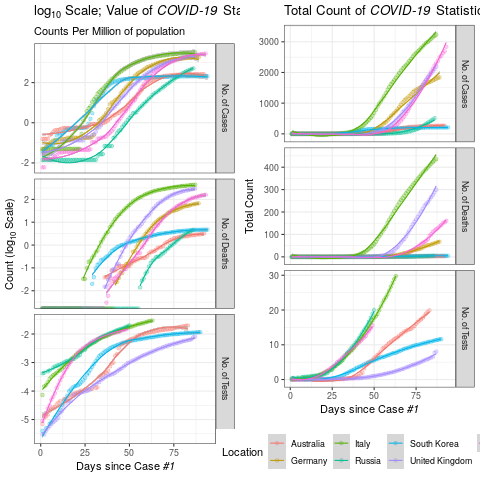
\includegraphics[width=18cm]{fgrid.png}
\caption{\label{fig:org542b788}Multi Scatter Plot of \emph{COVID-19} Metrics.}
\end{figure}

\subsection{Advantages compared to other methods}
\label{sec:orgb1bf3c2}
\begin{itemize}
\item The advantage to a log-scaled plot is that it allows rates of change to be
compared between countries
\item Making the Data Relative to the day of the first infection allows individual
countries to be compared in terms of there response
\end{itemize}
\subsection{Disasadvantages}
\label{sec:org29ecbad}
\begin{itemize}
\item A log-scaled plot can be misleading if it is not made clear, this is particularly
true for readers who have limited mathematical training.
\begin{itemize}
\item For this reason a plot without log-scaling was included and the axis were
labelled accordingly
\end{itemize}
\item Making Data relative to the day of the first infection may not make clear that
certain countries had \emph{forewarning} of the disease by virtue of the delay.
\end{itemize}
\subsection{Discussion on analysis results}
\label{sec:orgdc0628a}
Although the plots have been adjusted to reflect the date that the first cases were observed, it is possible that the disease began spreading before the first official case was reported, this is a belief held by some health officials in Italy.\cite{godin2020}

\subsubsection{Number of Cases}
\label{sec:orge8291b8}
This plot clearly suggests that the spread of the disease was the greatest both in rate and magnitude in Italy, some researchers belive that this is due simply to the fact that Italy has performed more tests. \cite{godin2020}
\subsubsection{Number of Deaths}
\label{sec:org40c1895}
Italy has had the highest amount of deaths despite it's higher rates of testing,
it is not clear why this is the case though. A study by \emph{IQAir} found that 25\% of the
most air-polluted European countries were located within Italy \cite{iqair2019}
and such pollution has been found to be correlated with higher rates of death
resulting from viral respiratory infection,
\cite{ciencewicki2007,croft2019,zhang2019} this could help explain some of the discrepancy but more research into the unique vulnerabilities of Italy is certainly warranted.

The Visualisation suggests that Russia has had the fewest number of deaths related to \emph{COVID-19}, however Moscow's Mayor, Sergei Sobyanin suggested that the official number of infections is likely much lower than reality, a sentiment echoed by Russia's \emph{Doctor's Alliance} ( which is essentially a doctors union). \cite{dole2020}

Dispensing with The view that Russia's figures are reliable it is clear that
Australia and South Korea have the lowest number of cases overall, while
Australia's success can be attributed to it's relative isolation and unique
quarantine requirements,
\cite{departmentofagrigulturewaterandtheenvironmentaustralia2019} combined with
lockdown's implemented early in the pandemic (with respect to Australia's first
case) \cite{willis2020} the success of South Korea Appears to be related more
appropriatley with the aggressive action taken by the country to contact trace the spread of the disease. \cite{thompson2020}

It appears that the number of deaths is more closely correlated with the number of cases than the number of tests, however it is not clear what the effect of testing is on the number of new cases.
\subsubsection{Number of Tests}
\label{sec:orgb87d931}
The visualisation also suggests that Italy and the US have undertaken the highest rates of testing, per capita, this
however does not appear to have influeced the rates of death or spread of cases significantly, indicating that measuring a countries response to the disease cannot be meaured merely by considering the rate of testing.


\subsection{Discussion on other Aspects}
\label{sec:org3171162}
\begin{itemize}
\item A potential improvement to this visualisation would be to plot many countries, say 30 but greyscale those countries and only apply colour to countries of interest, this would provide background information relative to those observations but not overwhelm the reader, this is a suggestion made by Andy Kirk in his \emph{Visualising Data} blog  \cite{kirk2015}.
\end{itemize}
\subsection{Literature review of related work}
\label{sec:org37574a5}
As mentioned in section \ref{orgb846a90} the use of the log-scaled and date-adjusted plot
was implemented by \emph{John Hopkins University} in a visualisation published in
\emph{The Guardian} newspaper \cite{gutierrez2020}.


NSW Health created a visualisation of cases acquired over time using a barchart
in a way that resembles a histogram, \cite{nswhealth2020} this plot is very easy
to interpret and clearly demonstrates the success of NSW in \emph{flattening the
curve}, this visualisation could have been implemented for this data as demonstrated in listing \ref{orgeb27ca5} and shown in figure \ref{fig:org244afa4} for different countries in a similar fashion, this however was not effective for comparing countries and so was not pursued.


\begin{listing}[htbp]
\begin{minted}[]{r}
#+begin_src
interested_locations <- c("Australia", "USA", "Italy", "Germany", "Russia", "South Korea", "United Kingdom")
cv <- covid %>%
  dplyr::filter(location %in% interested_locations)

ggplot(fortify(cv), aes(x = as.Date(date), y = new_cases_per_million, fill = location)) +
  geom_col(col = "grey") +
  labs(x = "Date", y = "New Cases Per Million") +
   theme(axis.text.x = element_text(angle = 90, hjust = 1)) +
  theme_bw()
\end{minted}
\caption{\label{orgeb27ca5}Use \texttt{ggplot} to create a bar chart}
\end{listing}


\begin{figure}[htbp]
\centering
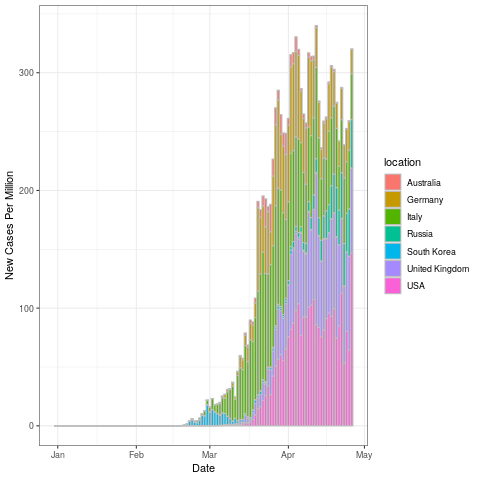
\includegraphics[width=10cm]{barex.png}
\caption{\label{fig:org244afa4}Bar Chart of cases over time for various locations}
\end{figure}


\section{Appendix}
\label{sec:orgb5a39e8}
PROPERTIES:
:ID:       84c19d03-8ab7-4793-a86d-e861e1bffe2b
\begin{figure}[htbp]
\centering
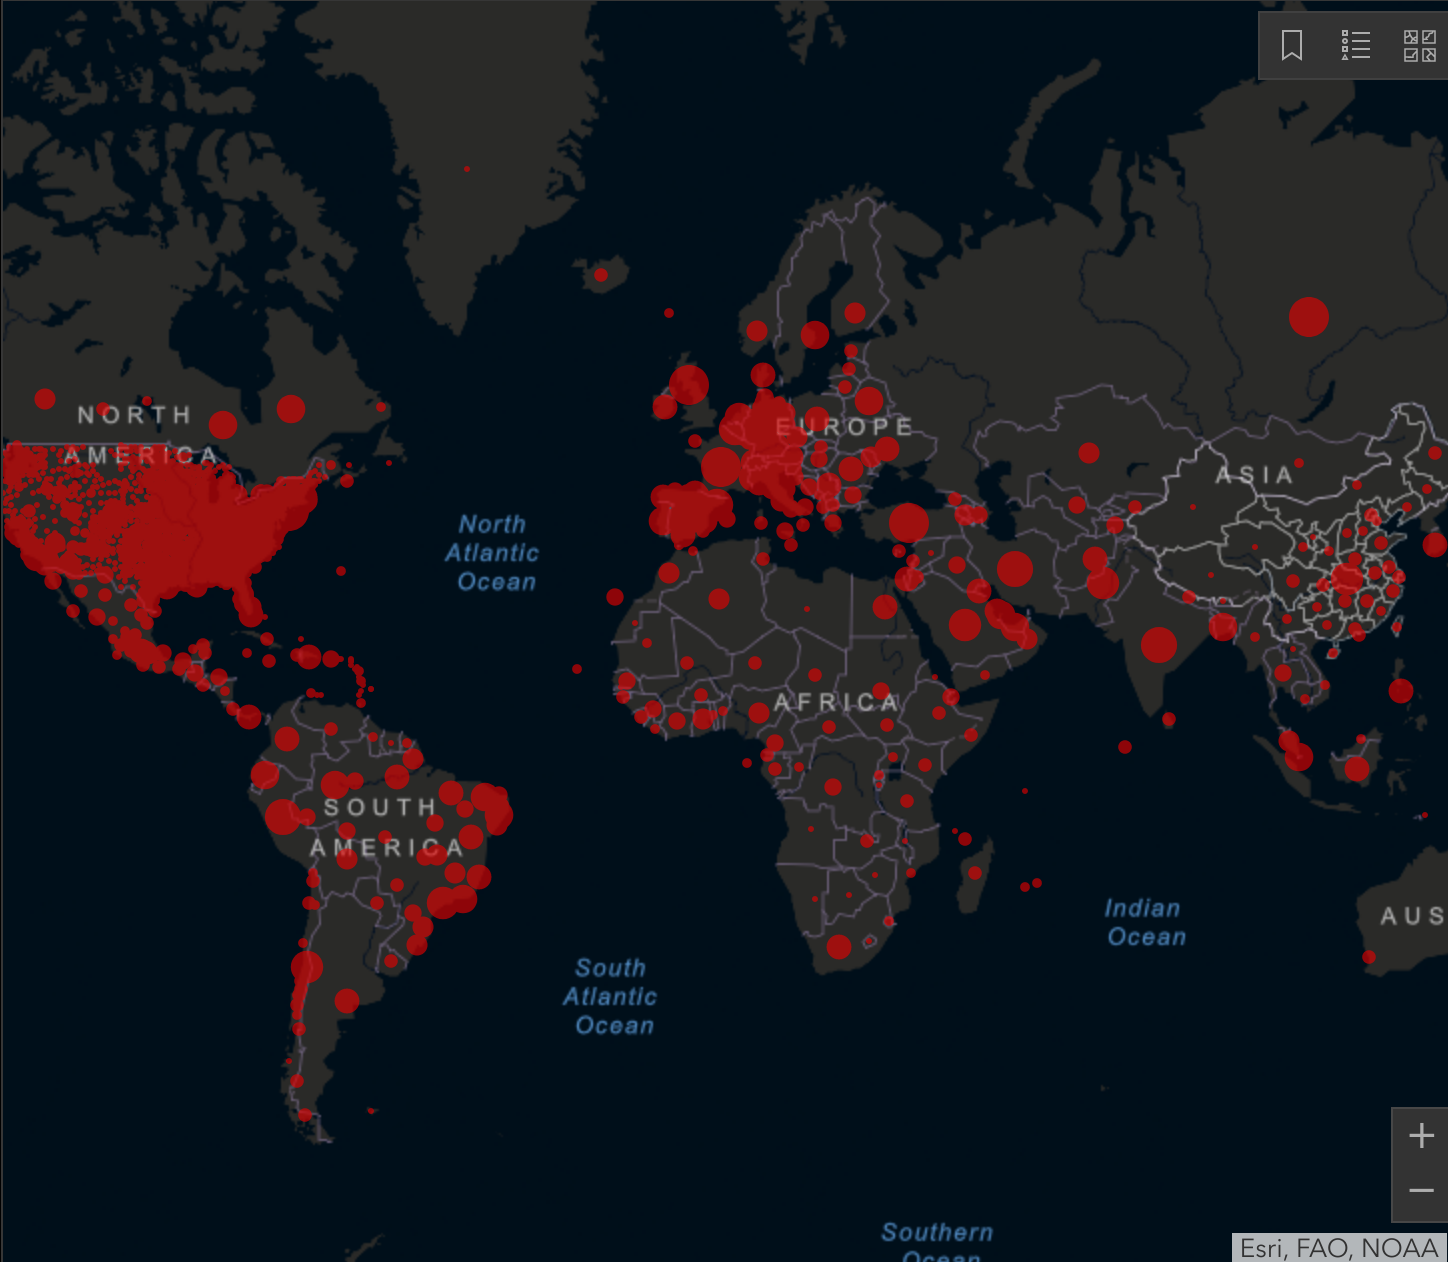
\includegraphics[width=8cm]{hopinScreen.png}
\caption{\label{fig:org2e5afd2}John Hopkins Bubble Chart \cite{2020o}}
\end{figure}


\begin{figure}[htbp]
\centering
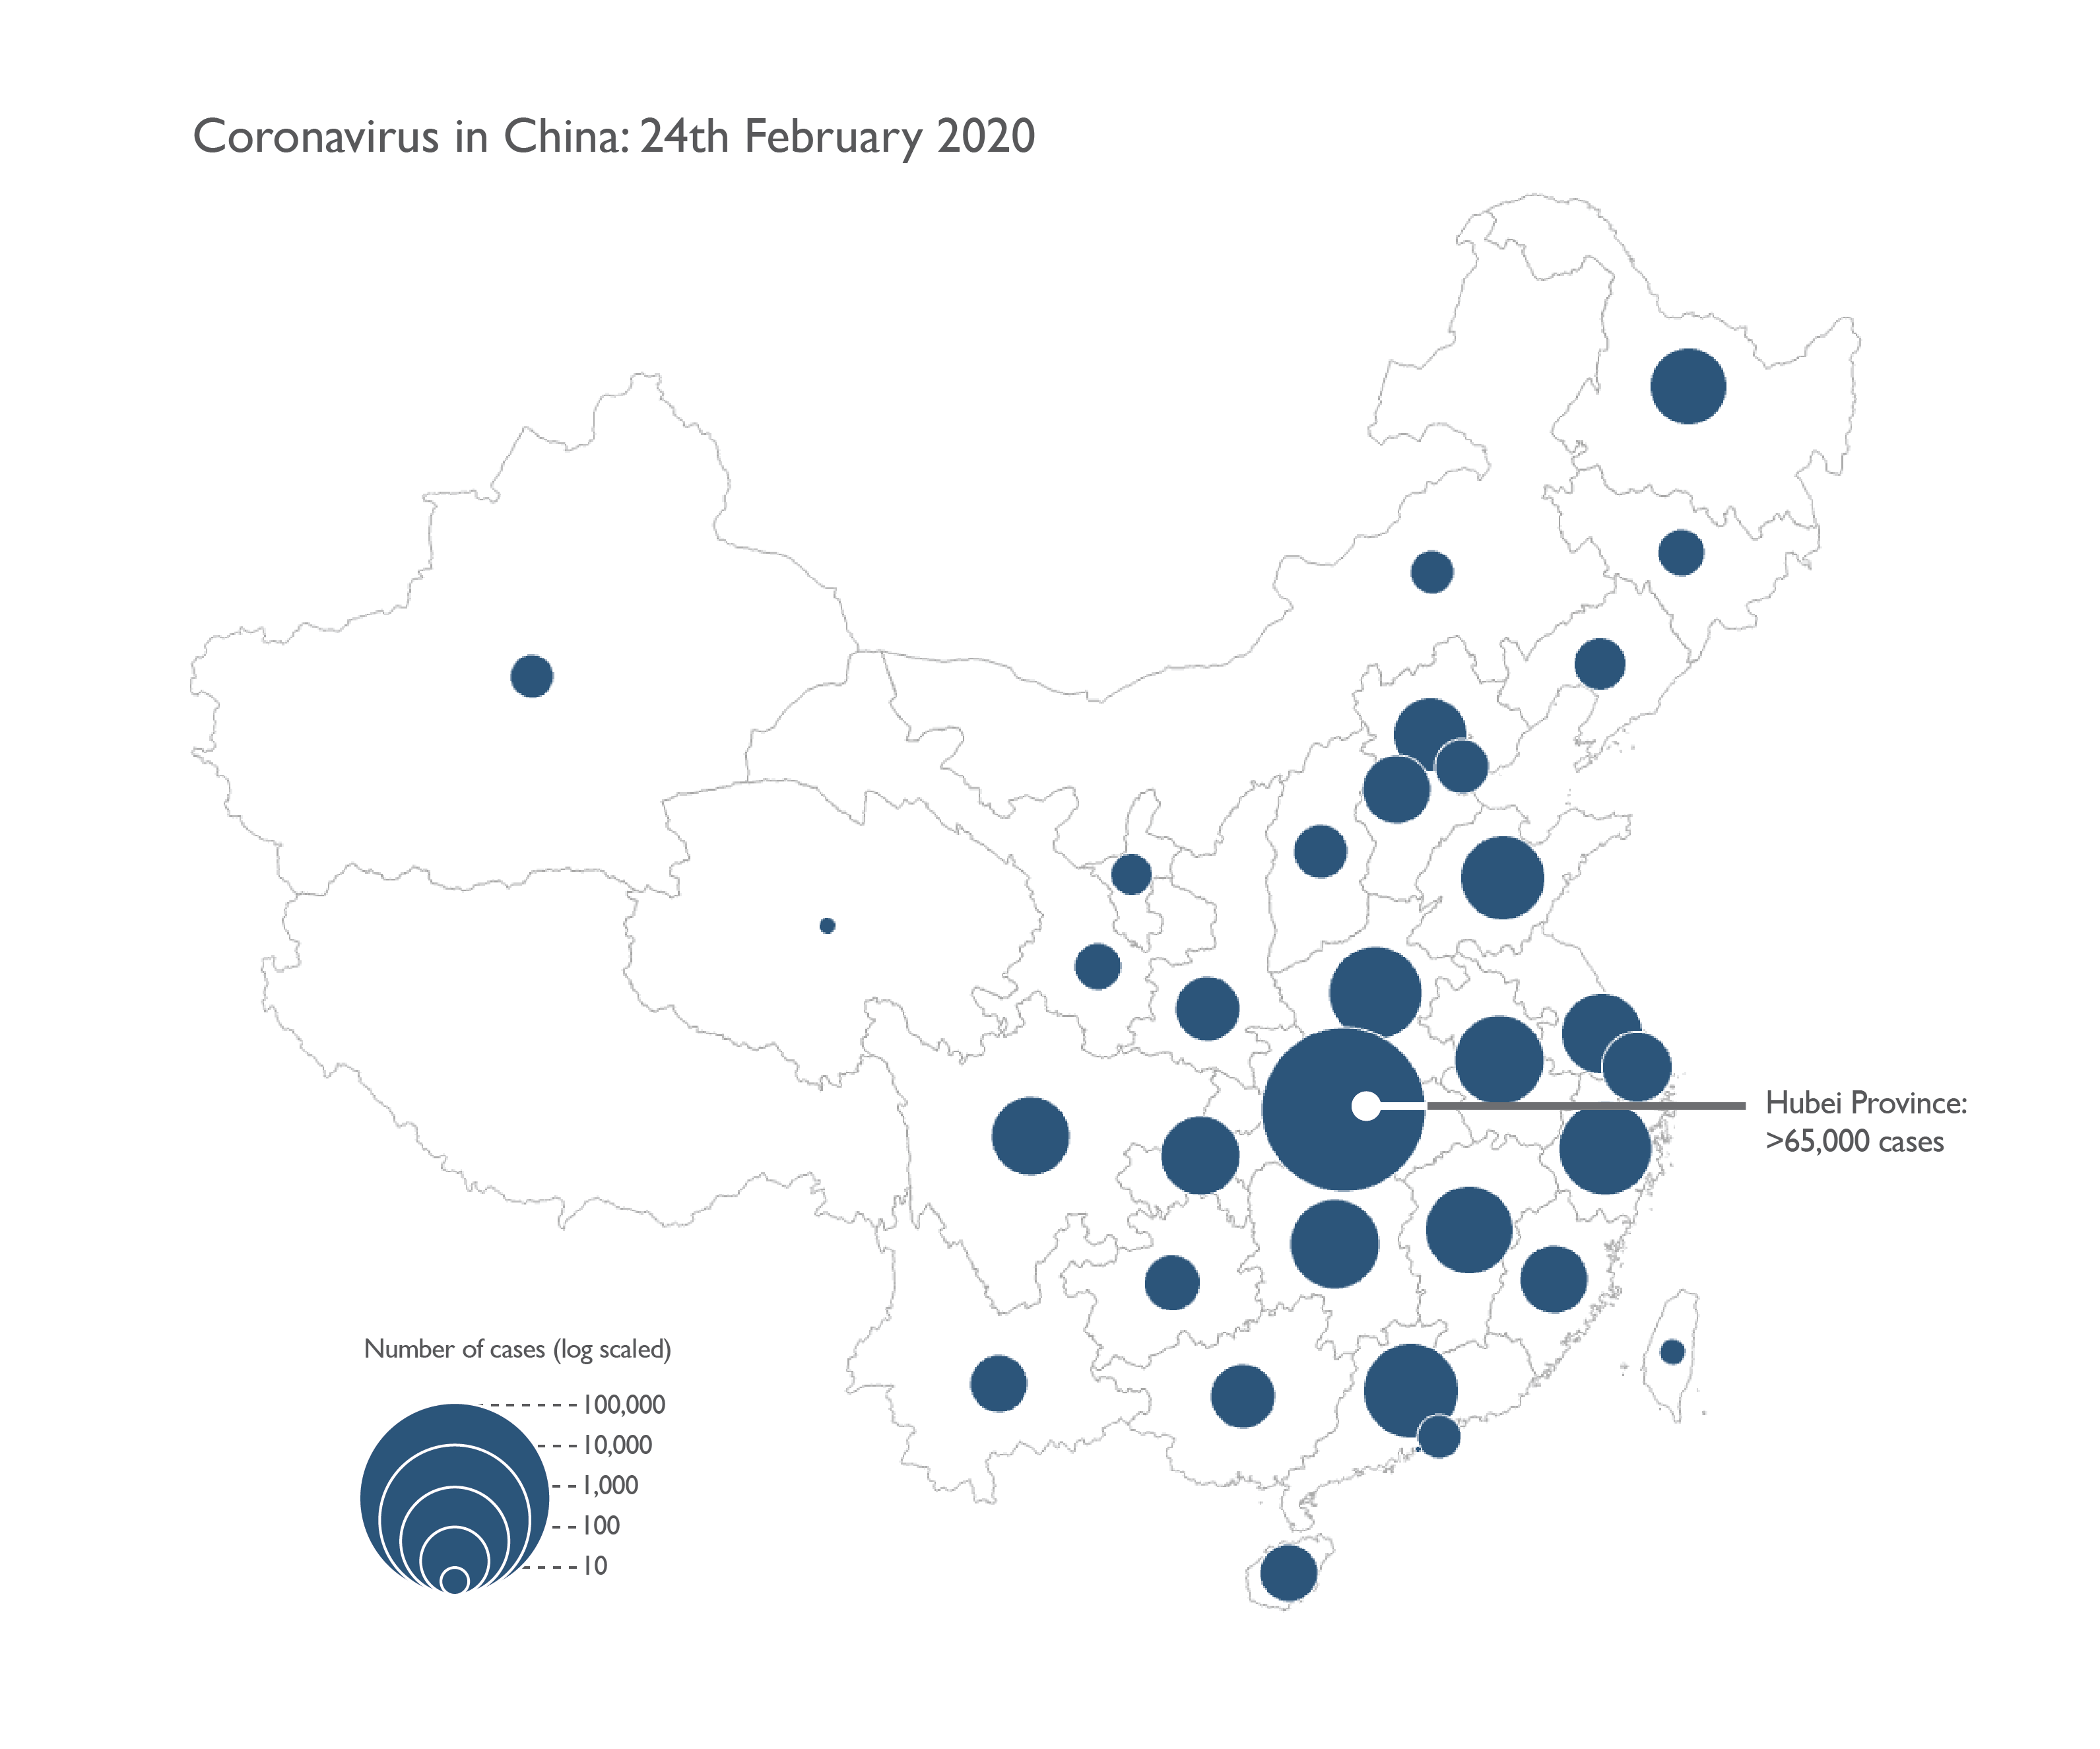
\includegraphics[width=10cm]{proppymap2.png}
\caption{\label{fig:orge888b39}Bubble Plot Chart produced by Field in his blog \cite{field2020}}
\end{figure}


\begin{figure}[htbp]
\centering
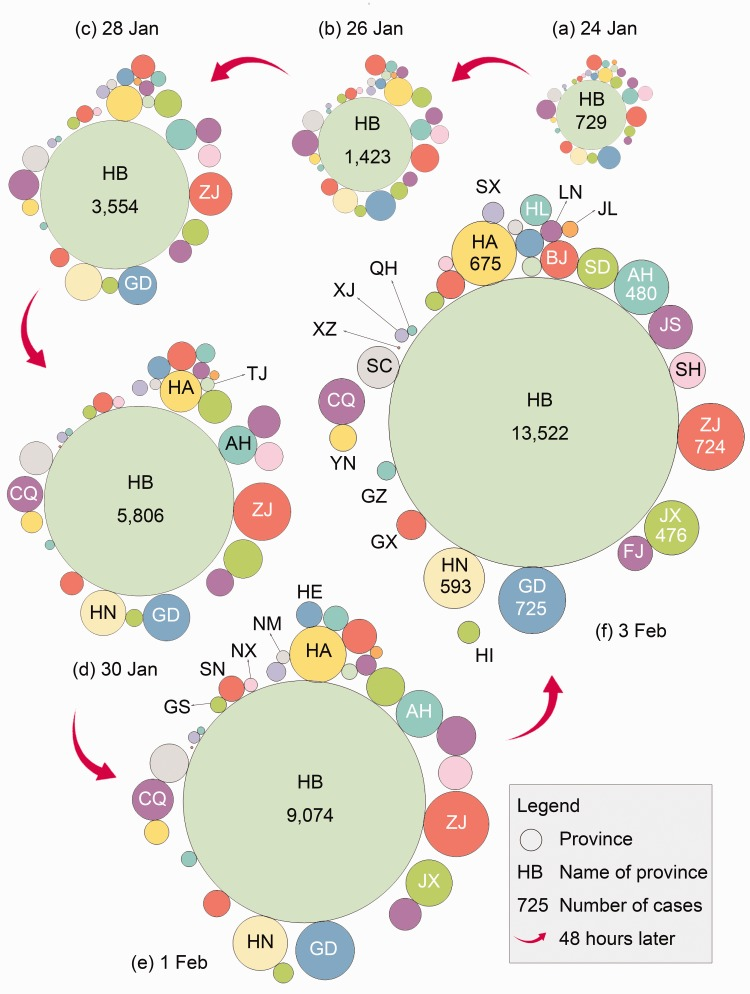
\includegraphics[width=10cm]{cartogramStudy.jpg}
\caption{\label{fig:orgb7dd52e}Cartogram of \emph{COVID-19} spread \cite{gao2020}}
\end{figure}

\begin{listing}[htbp]
\begin{minted}[]{r}
citation()
citation("ggplot2")


##  To cite R in publications use:
##
##    R Core Team (2020). R: A language and environment for statistical
##    computing. R Foundation for Statistical Computing, Vienna, Austria.
##    URL https://www.R-project.org/.
##
##  A BibTeX entry for LaTeX users is
##
##    @Manual{,
##      title = {R: A Language and Environment for Statistical Computing},
##      author = {{R Core Team}},
##      organization = {R Foundation for Statistical Computing},
##      address = {Vienna, Austria},
##      year = {2020},
##      url = {https://www.R-project.org/},
##    }
##
##  We have invested a lot of time and effort in creating R, please cite it
##  when using it for data analysis. See also ‘citation("pkgname")’ for
##  citing R packages.
##
##  To cite ggplot2 in publications, please use:
##
##    H. Wickham. ggplot2: Elegant Graphics for Data Analysis.
##    Springer-Verlag New York, 2016.
##
##  A BibTeX entry for LaTeX users is
##
##    @Book{,
##      author = {Hadley Wickham},
##      title = {ggplot2: Elegant Graphics for Data Analysis},
##      publisher = {Springer-Verlag New York},
##      year = {2016},
##      isbn = {978-3-319-24277-4},
##      url = {https://ggplot2.tidyverse.org},
##    }
\end{minted}
\caption{\label{orgc761d89}Generate Citation for \textbf{\emph{R}} programming Language}
\end{listing}

\section{References}
\label{sec:org63fafc1}
\end{document}
